\problemname{Mineral deposits}

\illustration{.3}{img/turnbull.jpg}{Eroding mud face exposing new minerals. Photo: Michael D.\ Turnbull, licence: CC BY-SA.}

\noindent
% You handle signal processing for an extra-terrestrial mining company, and your vessel is currently approaching an asteroid.
% Preliminary scans show the presence of $k$~mineral deposits on the asteroid, but their precise locations are unknown.
Ви займаєтеся обробкою сигналів для компанії з видобутку космічних руд, а Ваше судно наразі підходить до астероїда.
Попередні сканування показують наявність $k$ родовищ мінералів на астероїді, але їх точні місця невідомі.

\medskip

% The surface of the asteroid can be seen as a grid of integer coordinates.
% Each of the mineral deposits is located at unknown integer coordinates such that the $i$th deposit has coordinates $(x_i, y_i)$ with
% $-b \le x_i \le b$ and $-b\le y_i \le b$ %constraint:depositcoords
% for some integer $b$ corresponding to the size of your initial scan.
Поверхня астероїда може бути описана сіткою цілих координат.
Кожне мінеральне родовище знаходиться в невідомих цілих координатах, таких що $i$-те родовище має координати $(x_i, y_i)$ з обмеженнями
$-b \le x_i \le b$ та $-b\le y_i \le b$ %constraint:depositcoords
для деякого цілого числа $b$, яке відповідає розміру Вашого початкового сканування.

% To determine the precise locations of the mineral deposits, you may send probes to the surface of the asteroid.
% The probes are sent out in waves of several probes at once.
Для визначення точних координат мінеральних родовищ Ви можете відправляти зонди на поверхню астероїда.
Зонди відправляються хвилею з декількох зондів одночасно.

% Say you sent a wave of $d$~probes to the surface at coordinates $(s_j,t_j)$ for $1\leq j\leq d$.
% When a probe arrives at its coordinates, it determines the Manhattan distances to each of the $k$~mineral deposits and sends the distances back to the ship.
% All data packets arrive at the same time, and it is not possible to determine which probes returned which distances.
% Thus the wave returns the $k\cdot d$ integer distances
% \[|x_i-s_j| + |y_i - t_j| \qquad\text{for all } i \in \{1,\ldots,k\} \text{ and } j \in\{ 1,\ldots,d\}\,.\]
Припустимо, що Ви відправили хвилю з $d$ зондів на поверхню з координатами $(s_j,t_j)$ для $1\leq j\leq d$.
Коли зонд досягає своїх координат, він визначає Манхеттенські відстані до кожного з $k$ мінеральних родовищ і відправляє відстані на судно.
Усі пакети даних надходять одночасно, і неможливо визначити, який зонд повернув які відстані.
Таким чином, хвиля повертає $k\cdot d$ цілих відстаней
\[|x_i-s_j| + |y_i - t_j| \qquad\text{для всіх } i \in \{1,\ldots,k\} \text{ and } j \in\{ 1,\ldots,d\}\,.\]

% You need to minimise the number of waves of probes that is sent to the surface.
Вам потрібно зменшити кількість хвиль зондів, що відправляються на поверхню.


% \section*{Interaction}
\section*{Взаємодія}


% This is an interactive problem.
% Interaction begins with you reading a single line containing three integers $b$, $k$, and $w$:
% the grid's boundary~$b$,
% the number~$k$ of mineral deposits,
% and the maximum number~$w$ of waves you may send.
Це інтерактивна задача.
Взаємодія починається з того, що Ви отримуєте один рядок, який містить три цілих числа $b$, $k$ і $w$:
межу сітки~$b$,
кількість мінеральних родовищ~$k$,
та максимальну кількість~$w$ хвиль, які ви можете відправити.

% You then ask at most $w$ queries, each corresponding to a wave.
% A query consists of \texttt{?} followed by $2d$ integers separated by space, such as ``\texttt{?} $s_1$ $t_1$ $\cdots$ $s_d$ $t_d$'', where the number~$d$ of probes in this wave must satisfy
% $1\leq d\leq 2000$. % constraint:wavesize
% The values $(s_i,t_i)$ are interpreted as the coordinates of the $i$th probe and must satisfy
% $-10^8 \leq s_i \leq 10^8$ and $-10^8 \leq t_i \leq 10^8$. % constraint:probecoordinates
% The response is a single line with $k \cdot d$ integers in non-decreasing order: all pairs of Manhattan distances between the mineral deposits and the probe coordinates.
% The total number of probes across all waves may not exceed
% $2\cdot 10^4.$ % constraint:totalprobes
Далі Ви можете задати не більше, ніж $w$ запитів, кожен з яких відповідає хвилі зондів.
Запит складається з \texttt{?}, за яким слідують $2d$ цілих чисел, розділених пробілом, таких як «\texttt{?} $s_1$ $t_1$ $\cdots$ $s_d$ $t_d$», де кількість зондів у цій хвилі, $d$, повинна задовольняти
$1\leq d\leq 2000$. % constraint:wavesize
Значення $(s_i,t_i)$ трактуються як координати $i$-го зонда і повинні задовольняти
$-10^8 \leq s_i \leq 10^8$ і $-10^8 \leq t_i \leq 10^8$. % constraint:probecoordinates
Відповідь є одним рядком з $k \cdot d$ цілих чисел у неспадаючому порядку: всі пари Мангетенських відстаней між мінеральними родовищами та координатами зонда.
Загальна кількість зондів у всіх хвилях не може перевищувати
$2\cdot 10^4.$ % constraint:totalprobes

% Interaction ends with you printing a single line consisting of \texttt{!} followed by $k$ points $x_1, y_1, x_2, y_2, \ldots x_k, y_k$, separated by space.
% This must be your last line of output.
Взаємодія закінчується, коли Ви виводите один рядок, що складається з \texttt{!}, за яким слідують $k$ точок $x_1, y_1, x_2, y_2, \ldots x_k, y_k$, розділені пробілом.
Це має бути останнім рядком виводу.

% Your submission is considered correct if you print all locations of the mineral deposits.
% You may print them in any order.
Рішення вважатиметься правильним, якщо Ви виведете всі місця розташування мінеральних родовищ.
Ви можете виводити їх у будь-якому порядку.

% \section*{Constraints and Scoring}
\section*{Обмеження та оцінювання}

% We always have
Ми завжди маємо:
$1\leq b \leq 10^8$, % constraint:b
$1 \leq k \leq 20$, % constraint:k
% and
та
$2 \le w \le 10^4$. % constraint:w

% Your solution will be tested on a set of test groups, each worth a number of points.
% Each test group contains a set of test cases.
% To get the points for a test group you need to solve all test cases in the test group.
% Your final score will be the maximum score of a single submission.
Ваше рішення буде перевірено на наборі тестових груп, кожна з яких має свою кількість балів.
Кожна група тестів містить набір тестових прикладів.
Щоб отримати бали за групу тестів, потрібно розв'язати всі тестові приклади в цій групі.
Ваш кінцевий бал буде максимальним балом, який Ви отримали за одне відправлення.

\medskip
\begin{tabular}{lll}
% Group & Points & Constraints \\\hline
Група & Бали & Обмеження \\\hline
  $1$ & $9$ & $k = 1, w = 10^4$\\
  $2$ & $19$ & $w \ge 500$\\
  $3$ & $11$ & $w \ge 210$\\
  $4$ & $7$ & $w \ge 130$\\
  $5$ & $20$ & $w \ge 3$, $b \le 10^4$\\
  $6$ & $15$ & $w \ge 3$, $b \le 10^7$\\
%  $7$ & $19$ & \emph{No further constraints}
  $7$ & $19$ & \emph{Немає додаткових обмежень}
\end{tabular}

% \section*{Example}
\section*{Приклад}

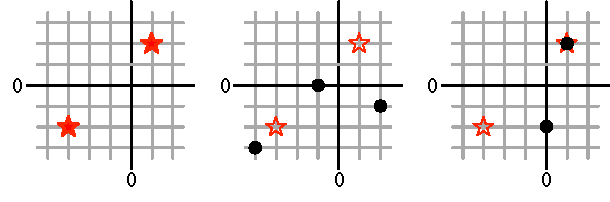
\includegraphics[width=.6\textwidth]{img/sample1.pdf}

% In this example, there are $k=2$ mineral deposits at positions $(1,2)$ and $(-3,-2)$, shown as red stars.
% In the first wave, you might send $d=3$ probes to $(-4,-3)$, $(-1, 0)$, and $(2,-1)$, shown as black dots.
% This wave would return the $6$ distances \[
%  2, 4, 4, 4, 6, 10\,.
% \]
У цьому прикладі є $k=2$ мінеральні родовища в позиціях $(1,2)$ та $(-3,-2)$, показаних червоними зірочками.
У першій хвилі Ви можете надіслати $d=3$ зонди до $(-4,-3)$, $(-1,0)$ та $(2,-1)$, показаних чорними крапками.
Ця хвиля поверне $6$ відстаней:
\[
  2, 4, 4, 4, 6, 10\,.
\]
% In the next wave, you might send $d=2$ probes to $(1,2)$ and $(0,-2)$.
% This wave would return the $4$ distances \[
%  0, 3, 5, 8\,.
% \]
У наступній хвилі ви можете надіслати $d=2$ зонди до $(1,2)$ та $(0,-2)$.
Ця хвиля поверне $4$ відстані: \[
  0, 3, 5, 8\,.
\]

